%%%%%%%%%%%%%%%%%%%%%%%%%%%%%%%%%%%%%%%%
\chapter{Metodología}
%%%%%%%%%%%%%%%%%%%%%%%%%%%%%%%%%%%%%%%%

El presente capítulo describe el proceso metodológico empleado para identificar, seleccionar y analizar la literatura sobre técnicas de \textit{fine-tuning} para \textit{Large Language Models}. Se adopta el protocolo PRISMA 2020 \parencite[p.~796]{page2021prisma}, un estándar para la conducción y reporte de revisiones sistemáticas que organiza el proceso en cuatro fases secuenciales: identificación de registros mediante búsqueda en bases de datos, cribado por título y resumen, evaluación de elegibilidad en texto completo, e inclusión del corpus definitivo. La adopción de este protocolo garantiza que cada decisión de inclusión o exclusión quede documentada de forma explícita y reproducible.

%%%%%%%%%%%%%%%%%%%%%%%%%%%%%%%%%%%%%%%%
\section{Estrategia de búsqueda}

La estrategia de búsqueda se diseñó siguiendo el marco PICO adaptado a revisiones de NLP, donde la población corresponde a \textit{Large Language Models}, la intervención a las técnicas de \textit{fine-tuning} en scope, la comparación a estudios con evaluación cuantitativa, y el resultado a métricas de rendimiento reportadas. A partir de este marco se definieron cuatro grupos de términos de búsqueda: términos de adaptación (\textit{fine-tuning}, \textit{finetuning}, \textit{fine tuning}), términos de modelo (\textit{large language model}, \textit{LLM}), términos de técnica (LoRA, \textit{low-rank adaptation}, \textit{adapter}, \textit{prefix tuning}, \textit{prompt tuning}, RLHF, DPO, \textit{parameter-efficient}, PEFT) y términos de evaluación (\textit{evaluation}, \textit{benchmark}, \textit{comparison}, \textit{empirical}, \textit{experimental}).

La búsqueda sistemática se realizó en la base de datos Scopus, seleccionada por su cobertura amplia de literatura académica en ciencias de la computación y procesamiento de lenguaje natural. La búsqueda se ejecutó sobre títulos, resúmenes y palabras clave mediante el siguiente \textit{query string}:

\begin{lstlisting}[basicstyle=\ttfamily\scriptsize]
TITLE-ABS-KEY(
  ("fine-tuning" OR "finetuning" OR "fine tuning")
  AND ("large language model" OR "large language models"
       OR "LLM" OR "LLMs")
  AND (
    "LoRA" OR "low-rank adaptation" OR
    "adapter" OR "adapters" OR
    "prefix tuning" OR "prompt tuning" OR
    "RLHF" OR "reinforcement learning from human feedback" OR
    "DPO" OR "direct preference optimization" OR
    "parameter-efficient" OR "PEFT"
  )
  AND (
    "evaluation" OR "benchmark" OR "benchmarking" OR
    "comparison" OR "comparative" OR
    "empirical" OR "experimental"
  )
)
AND PUBYEAR > 2019 AND PUBYEAR < 2026
AND DOCTYPE(ar)
AND OA(all)
AND LANGUAGE(english)
\end{lstlisting}

Se aplicaron los siguientes filtros directamente en la plataforma: período de publicación 2020-2025, tipo de documento restringido a artículos de revista, acceso abierto e idioma inglés. La búsqueda retornó 140 registros, los cuales fueron sometidos al proceso de selección descrito en la sección siguiente.
%%%%%%%%%%%%%%%%%%%%%%%%%%%%%%%%%%%%%%%%
\section{Proceso de selección de estudios}

El proceso de selección se estructuró en dos fases secuenciales de cribado siguiendo el protocolo PRISMA 2020. La Figura~\ref{fig:prisma} presenta el diagrama de flujo completo con los registros procesados en cada etapa. Todo el proceso fue implementado mediante código Python con llamadas estructuradas a APIs de modelos de lenguaje, garantizando reproducibilidad y trazabilidad de cada decisión.

\begin{figure}[H]
\centering
\caption{Diagrama de flujo PRISMA 2020 del proceso de selección de estudios}
\label{fig:prisma}
% Nodo naranja separado del tikzpicture para evitar problemas de ancho
\noindent\tikz\node[draw, rectangle, rounded corners=4pt, fill=orange!45, thick,
  text width=\textwidth-2\pgflinewidth-2\fboxsep,
  minimum height=9mm, align=center, font=\small\bfseries,
  inner ysep=6pt]
  {Identificación de estudios a través de bases de datos y registros};

\vspace{5mm}
\resizebox{\textwidth}{!}{%
\tikzset{every path/.style={}}%
\begin{tikzpicture}[node distance=8mm and 12mm, start chain=going below,
    arrow/.style={-latex, thick},
    every node/.style={font=\scriptsize}]
\node[draw, rectangle, align=center, minimum height=12ex,
      text width=7cm, outer sep=0pt,
      on chain] (ident)
    {Registros identificados a partir de Scopus:\\
     Bases de datos (n\,=\,140)\quad Registros (n\,=\,0)};
\node[draw, rectangle, align=center, minimum height=12ex,
      text width=7cm, outer sep=0pt, on chain] (crib)
    {Registros cribados\\ (n\,=\,140)};
\node[draw, rectangle, align=center, minimum height=12ex,
      text width=7cm, outer sep=0pt, on chain] (eleg)
    {Informes evaluados para elegibilidad\\ (n\,=\,101)};
\node[draw, rectangle, align=center, minimum height=12ex,
      text width=7cm, outer sep=0pt, on chain] (incl)
    {Estudios incluidos en la revisión (n\,=\,84)\\
     Informes de estudios incluidos (n\,=\,84)};
\draw[arrow] (ident.south) -- (crib.north);
\draw[arrow] (crib.south)  -- (eleg.north);
\draw[arrow] (eleg.south)  -- (incl.north);
\node[draw, rectangle, align=center, minimum height=12ex,
      text width=5.5cm, outer sep=0pt,
      right=12mm of ident] (eprev)
    {Registros eliminados antes del cribado:\\
     Duplicados (n\,=\,0)\quad No elegibles (n\,=\,0)\\
     Otras razones (n\,=\,0)};
\node[draw, rectangle, align=center, minimum height=12ex,
      text width=5.5cm, outer sep=0pt,
      right=12mm of crib] (excl1)
    {Registros excluidos (n\,=\,39):\\
     No superaron cribado por\\
     título y resumen};
\node[draw, rectangle, align=center,
      text width=5.5cm, outer sep=0pt,
      right=12mm of eleg] (excl2)
    {Informes excluidos (n\,=\,17):\\
     Q1: Sin métricas cuantitativas (n\,=\,1)\\
     Q2: Técnica fuera del alcance (n\,=\,7)\\
     Q4: Tarea o modelo no especif.\ (n\,=\,16)\\
     Q5: No es estudio empírico orig.\ (n\,=\,1)};
\draw[arrow] (ident.east) -- (eprev.west);
\draw[arrow] (crib.east)  -- (excl1.west);
\draw[arrow] (eleg.east)  -- (excl2.west);
\path let \p1=(ident.north), \p2=(ident.south)
in node[draw, rounded corners, fill=blue!35, thick,
        inner sep=2pt, minimum width=7mm, minimum height={\y1-\y2},
        align=center, anchor=north east] at ([xshift=-2mm]ident.north west)
   {\rotatebox{90}{\textbf{\scriptsize Identificación}}};
\path let \p1=(crib.north), \p2=(eleg.south)
in node[draw, rounded corners, fill=blue!35, thick,
        inner sep=2pt, minimum width=7mm, minimum height={\y1-\y2},
        align=center, anchor=north east] at ([xshift=-2mm]crib.north west)
   {\rotatebox{90}{\textbf{\scriptsize Cribado}}};
\path let \p1=(incl.north), \p2=(incl.south)
in node[draw, rounded corners, fill=blue!35, thick,
        inner sep=2pt, minimum width=7mm, minimum height={\y1-\y2},
        align=center, anchor=north east] at ([xshift=-2mm]incl.north west)
   {\rotatebox{90}{\textbf{\scriptsize Incluidos}}};
\end{tikzpicture}%
}
\begin{flushleft}
\footnotesize
\textit{Nota.} Elaborado siguiendo las directrices de \textcite{page2021prisma}.
\end{flushleft}
\end{figure}

\subsection{Fase 1: Cribado de título y resumen}

Los 140 registros identificados en Scopus fueron evaluados mediante un sistema automatizado de votación por mayoría implementado con GPT-4o-mini. Cada registro recibió cuatro evaluaciones independientes, cada una con un perfil de evaluador distinto: experto en revisiones sistemáticas de NLP, revisor académico senior especializado en LLMs, investigador en aprendizaje automático, y experto en evaluación metodológica. La variación de perfiles buscó reducir sesgos al forzar perspectivas independientes sobre el mismo registro.

Cada evaluador respondió de manera binaria si el registro cumplía simultáneamente los tres criterios de inclusión:

\begin{itemize}
    \item \textbf{C1}: El artículo trata sobre \textit{fine-tuning} de \textit{Large Language Models} (GPT, LLaMA, Mistral, Claude, Falcon, BLOOM, OPT). Se excluyen modelos \textit{encoder-only} como BERT o RoBERTa.
    \item \textbf{C2}: El artículo evalúa al menos una de las nueve técnicas objetivo: \textit{Full Fine-Tuning}, SFT, LoRA, QLoRA, \textit{Adapter Layers}, \textit{Prefix Tuning}, \textit{Prompt Tuning}, RLHF o DPO.
    \item \textbf{C3}: El artículo reporta evaluación empírica con métricas cuantitativas (\textit{accuracy}, F1, BLEU, ROUGE, \textit{perplexity} o \textit{benchmark scores}).
\end{itemize}

La decisión final se determinó por mayoría simple: con tres o más votos favorables el registro fue aceptado, con dos o menos fue rechazado. Los registros con empate exacto fueron marcados para revisión manual. De los 140 registros evaluados, 101 superaron esta fase y avanzaron a la evaluación de texto completo. Los 39 registros restantes fueron excluidos por no cumplir los criterios de inclusión.

\subsection{Fase 2: Evaluación de texto completo}

Los 101 artículos fueron evaluados en texto completo mediante Claude Sonnet 4.6, utilizando \textit{tool use} estructurado para garantizar respuestas en formato JSON validado. El texto completo de cada PDF fue extraído automáticamente mediante PyMuPDF y enviado al modelo junto con cinco criterios de elegibilidad:

\begin{itemize}
    \item \textbf{Q1}: ¿El artículo reporta resultados numéricos explícitos usando \textit{accuracy}, F1, \textit{precision}, \textit{recall}, BLEU, ROUGE u otros \textit{scores} de \textit{benchmarks} estándar?
    \item \textbf{Q2}: ¿El artículo implementa al menos una técnica en scope con evidencia de aplicación real, reportando \textit{optimizer}, \textit{dataset} y \textit{training steps} o \textit{epochs}?
    \item \textbf{Q3}: ¿El artículo identifica el \textit{dataset} utilizado especificando nombre y dominio de aplicación?
    \item \textbf{Q4}: ¿El artículo especifica tanto la tarea NLP realizada como la arquitectura del modelo base utilizado?
    \item \textbf{Q5}: ¿Es un estudio empírico original con resultados experimentales propios, excluyendo \textit{surveys}, revisiones de literatura y artículos teóricos?
\end{itemize}

Los criterios Q1, Q2, Q4 y Q5 operaron con lógica eliminatoria directa: un resultado negativo en cualquiera resultó en exclusión inmediata. El criterio Q3 recibió tratamiento especial: un resultado negativo derivó en revisión manual en lugar de exclusión directa, dado que estudios de dominio aplicado pueden describir correctamente su corpus sin nombrar un \textit{dataset} público estándar. De los 101 artículos evaluados, 84 fueron incluidos y 17 excluidos. La Figura~\ref{fig:criterios} desglosa las exclusiones por criterio, evidenciando que Q4 fue el más restrictivo con 16 exclusiones, seguido de Q2 con 7. Los criterios Q1 y Q5 generaron una exclusión cada uno, mientras que Q3 no produjo exclusiones directas dado que los casos negativos derivaron en revisión manual.

\begin{figure}[H]
    \centering
    \caption{Artículos excluidos por cada criterio de elegibilidad en la Fase 2 (n = 101)}
    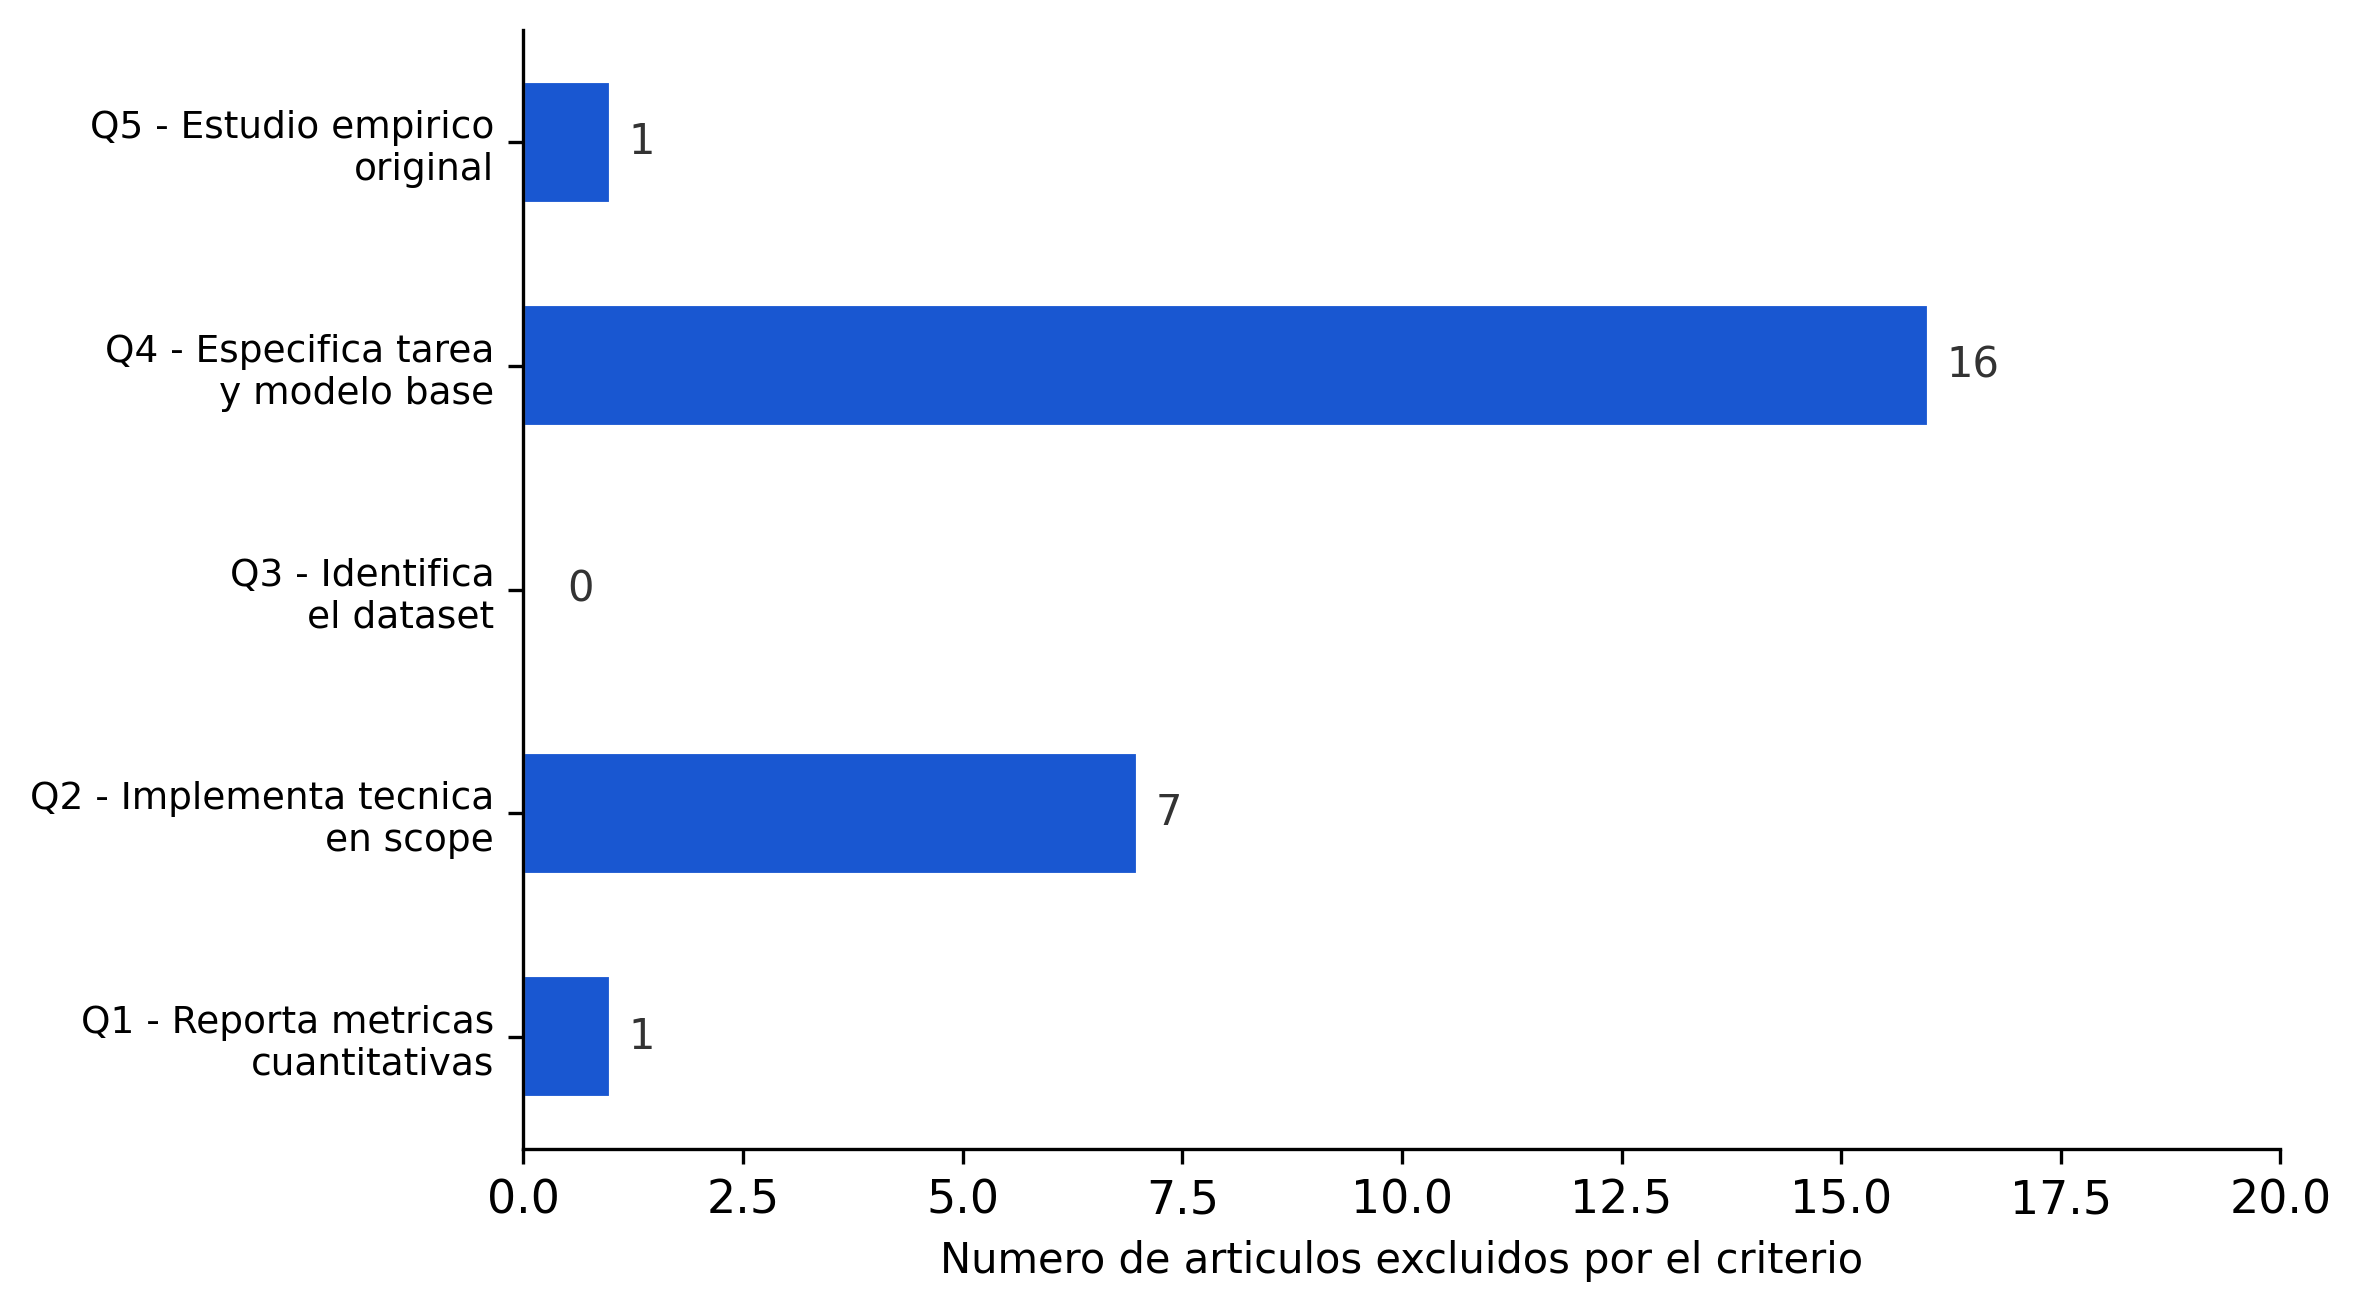
\includegraphics[width=0.85\linewidth]{Imagenes/fig1_criterios_elegibilidad.png}
    \label{fig:criterios}
    \begin{flushleft}
    \footnotesize
    \textit{Nota.} El criterio Q3 no aparece con exclusiones directas porque los casos negativos derivaron en revisión manual. Los valores pueden sumar más de 17 si un mismo artículo no cumplió más de un criterio.
    \end{flushleft}
\end{figure}

%%%%%%%%%%%%%%%%%%%%%%%%%%%%%%%%%%%%%%%%
\section{Evaluación de calidad metodológica}

Los 84 estudios incluidos fueron sometidos a una evaluación de calidad metodológica mediante Claude Haiku 4.5, utilizando \textit{tool use} estructurado sobre el texto completo de cada artículo. Cada estudio fue evaluado según tres criterios en escala 0\,/\,0.5\,/\,1, con un score máximo de 3,0:

\begin{itemize}
    \item \textbf{QA1}: ¿El artículo reporta explícitamente las proporciones del \textit{split} train/test o los tamaños exactos de cada subconjunto?
    \item \textbf{QA3}: ¿El artículo reporta una configuración de entrenamiento completa incluyendo \textit{learning rate}, \textit{batch size}, \textit{epochs} y parámetros técnica-específicos?
    \item \textbf{QA4}: ¿El artículo caracteriza completamente el \textit{dataset} con nombre, dominio y tamaño?
\end{itemize}

Los scores obtenidos en esta evaluación se emplean como criterio de priorización interpretativa en la síntesis comparativa presentada en el capítulo de Resultados: los hallazgos provenientes de estudios con score alto (score $\geq$ 2,5) se priorizaron como soporte principal de los patrones transversales identificados, mientras que los hallazgos de estudios con calidad media se reportan en el análisis descriptivo pero no fundamentan las conclusiones comparativas.

%%%%%%%%%%%%%%%%%%%%%%%%%%%%%%%%%%%%%%%%
\section{Clasificación por dominio de aplicación}

Cada uno de los 84 estudios incluidos fue asignado a uno de cuatro dominios de aplicación definidos a priori. La clasificación se realizó de forma automatizada durante la Fase 3, como parte del mismo proceso de evaluación de calidad metodológica, utilizando el texto completo de cada artículo como insumo. Los criterios de asignación empleados fueron los siguientes:

\begin{itemize}
    \item \textbf{Salud y Biomedicina}: estudios cuya tarea principal involucra NLP clínico, registros médicos, texto biomédico, descubrimiento de fármacos, salud mental, radiología, genómica o datos de pacientes.
    \item \textbf{Ciencias Exactas y Computación}: estudios enfocados en generación de código, razonamiento matemático, ingeniería de software, verificación formal, tareas de programación, ciberseguridad o \textit{benchmarks} de ciencias de la computación.
    \item \textbf{Lenguaje y Humanidades}: estudios que abordan tareas generales de NLP como traducción, resumen, análisis de sentimiento, reconocimiento de entidades nombradas, respuesta a preguntas sobre corpus generales, lingüística, literatura o texto de redes sociales.
    \item \textbf{Industria y Negocios}: estudios con aplicaciones en finanzas, derecho, educación, atención al cliente, comercio electrónico, recursos humanos, logística o aplicaciones empresariales.
\end{itemize}

Cuando un estudio evaluaba múltiples tareas en dominios distintos, se asignó al dominio principal según la contribución declarada por los autores. Esta clasificación constituye el eje organizador del análisis comparativo presentado en el capítulo de Resultados.

%%%%%%%%%%%%%%%%%%%%%%%%%%%%%%%%%%%%%%%%
\section{Extracción de datos}

De cada uno de los 84 estudios incluidos en el corpus final se extrajeron datos estructurados mediante lectura directa del texto completo de cada artículo. Este proceso se realizó de forma independiente al pipeline de selección PRISMA descrito en las secciones anteriores. Como apoyo a la identificación inicial, se empleó un modelo de lenguaje (Claude, Anthropic) para localizar en cada artículo la técnica principal implementada, la tarea de aplicación y la presencia o ausencia de un \textit{baseline} de referencia explícito; los valores finales fueron verificados y registrados manualmente contrastando cada campo contra el texto original del artículo.

Los campos extraídos fueron los siguientes: técnica de \textit{fine-tuning} implementada, tarea y dominio de aplicación, métrica principal de evaluación, valor del \textit{baseline} de referencia y mejor resultado obtenido por el modelo evaluado. A partir de los dos últimos campos se calculó el incremento porcentual ($\Delta$\%) respecto al \textit{baseline}. Los campos no reportados explícitamente en el artículo fueron registrados como \textit{not reported}, sin inferencia ni estimación de valores ausentes.

Para que el cálculo de mejora relativa fuera metodológicamente válido, se aplicó un criterio de comparabilidad: un estudio se consideró comparable únicamente si los autores declaraban un \textit{baseline} único y explícito contra el cual comparar el resultado principal. Quedaron excluidos de la comparación cuantitativa los estudios que evaluaban múltiples modelos sin designar una referencia de comparación fija, y aquellos donde se presentaban resultados para más de un modelo \textit{fine-tuneado} sin indicar cuál constituía el resultado principal, impidiendo el cálculo de un incremento atribuible a la técnica de forma aislada. Bajo este criterio, 30 de los 84 estudios presentaron pares de valores comparables; los 54 restantes se reportan en el análisis descriptivo del corpus pero no contribuyen a la síntesis cuantitativa de mejora relativa.

%%%%%%%%%%%%%%%%%%%%%%%%%%%%%%%%%%%%%%%%
\section{Análisis de datos}

El análisis de datos se organizó en tres niveles complementarios sobre el corpus de 84 estudios incluidos.

El análisis descriptivo caracterizó el corpus mediante frecuencias de técnicas de \textit{fine-tuning}, distribución por dominio de aplicación, modelos base más utilizados y métricas de evaluación más frecuentes. Este nivel permitió identificar los patrones dominantes en la literatura reciente sobre \textit{fine-tuning} de LLMs.

El análisis comparativo sintetizó el rendimiento reportado por dominio de aplicación, comparando los resultados de cada estudio contra sus \textit{baselines} de referencia dentro de cada dominio. Dado que los estudios emplean métricas y \textit{datasets} heterogéneos, la comparación se realizó a nivel de mejora relativa sobre el \textit{baseline} en lugar de valores absolutos, permitiendo identificar patrones de efectividad por dominio independientes de la escala de cada métrica.

El análisis de calidad metodológica empleó los \textit{scores} obtenidos en la evaluación de calidad como criterio de priorización interpretativa: los hallazgos provenientes de estudios con \textit{score} alto (\textit{score} $\geq$ 2,5) se priorizaron como soporte principal de los patrones transversales identificados, mientras que los hallazgos de estudios con calidad media se reportan en el análisis descriptivo pero no fundamentan las conclusiones comparativas.